\documentclass[11pt,a4paper]{article}
\usepackage[margin=2.3cm]{geometry}
\usepackage{graphicx}
\usepackage{amsmath}
\usepackage{booktabs}
\usepackage{float}
\usepackage{xcolor}
\usepackage{listings}
\usepackage{hyperref}
\usepackage{caption}
\usepackage{enumitem}
\setlist{nosep}

\hypersetup{colorlinks=true, linkcolor=blue!50!black, urlcolor=blue!50!black}
\lstset{basicstyle=\ttfamily\small, breaklines=true, frame=single,
        backgroundcolor=\color{gray!8}, keywordstyle=\color{blue!60!black},
        commentstyle=\color{green!40!black}, columns=fullflexible}

% ---------- fill in your team here (used on the title page) ----------
\newcommand{\teamtable}{%
\begin{tabular}{ll}
\toprule
Name & Roll number \\
\midrule
Rahul Ahirwar & CS25BT011
\bottomrule
\end{tabular}}
\newcommand{\coursename}{Software Systems Lab}
\newcommand{\institute}{IIT Dharwad}
% ----------------------------------------------------------------------

\begin{document}

\begin{titlepage}
\centering
\vspace*{2cm}
{\Large \coursename{} -- Project Report\par}
\vspace{1cm}
{\Huge\bfseries CPU / Process Monitor\\[4pt] and Job Scheduler\par}
\vspace{1.5cm}

\vspace{1.5cm}

{\large \institute\par}
\vspace{0.5cm}
{\large November 2026\par}
\vfill
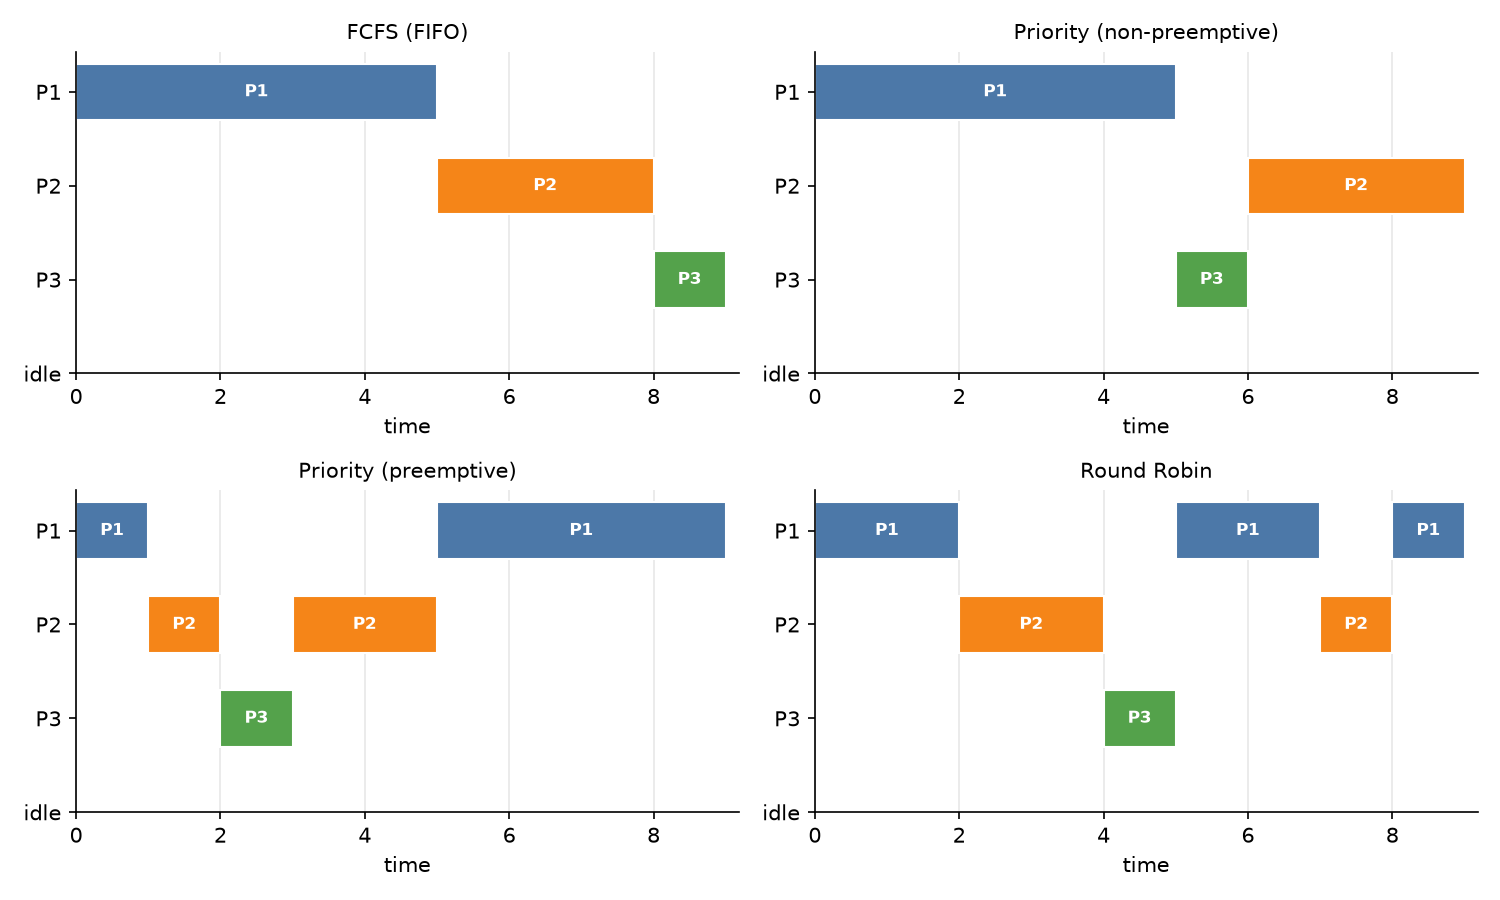
\includegraphics[width=0.75\textwidth]{gantt_all.png}
\end{titlepage}

\begin{abstract}
We built a desktop application in Python that watches the processes running on a
Unix machine (macOS/Linux) and also acts as a CPU scheduler. The monitor shows every
process with its CPU and memory use, draws the parent--child process tree and plots live
system graphs. The scheduler part runs First Come First Served (FCFS), Priority
(preemptive and non-preemptive) and Round Robin scheduling, draws Gantt charts and
computes waiting, turnaround and response time, throughput and CPU utilisation.
It can also schedule \emph{real} child processes by pausing and resuming them with the
Unix signals \texttt{SIGSTOP} and \texttt{SIGCONT}. Background work runs on threads so the
GUI never freezes. We used \texttt{cProfile} to find a bottleneck in our priority
scheduler and made it about 66--133 times faster with a heap. The project includes
26 unit tests, 7 bash scripts and a git history that follows the development.
\end{abstract}

\tableofcontents
\newpage

%=======================================================================
\section{Introduction}

An operating system runs hundreds of processes at the same time even though one CPU
core can only execute one of them at any instant. Two questions follow:
\begin{enumerate}
  \item \textbf{What is running right now?} This is answered by \emph{process monitoring}
        (tools like \texttt{top}, \texttt{ps} or Activity Monitor).
  \item \textbf{Who should run next?} This is answered by the \emph{CPU scheduler}.
\end{enumerate}
Our project answers both questions inside one application.

\subsection{Objectives}
\begin{itemize}
  \item List all processes with PID, PPID, user, state, CPU\%, memory and threads, and allow
        sending signals (terminate, kill, suspend, resume).
  \item Show the Unix process hierarchy as a tree.
  \item Plot CPU and memory usage live.
  \item Implement FCFS, Priority and Round Robin scheduling and compare them with statistics and Gantt charts.
  \item Schedule real operating-system processes with signals.
  \item Keep the GUI responsive using threads.
  \item Test, profile and automate the project, and track it with git.
\end{itemize}

\subsection{Course topics covered}
\begin{table}[H]
\centering
\begin{tabular}{lp{10cm}}
\toprule
Topic & Where it is used \\
\midrule
Unix process hierarchy & Process tree from PPID, fork/exec of child jobs, signals \\
Process monitoring & \texttt{psutil} snapshots, process states, system statistics \\
Threads & Monitor thread and scheduler thread, locks and queues \\
Python & Whole application, \texttt{unittest}, \texttt{cProfile} \\
GUI & Tkinter application with five tabs \\
Plotting & matplotlib: live graphs, Gantt charts, comparison charts \\
Bash & Seven automation scripts (setup, run, tests, profiling, docs, stress, demo) \\
Git & Step-by-step commit history \\
Profiling & \texttt{cProfile}, \texttt{pstats}, \texttt{/usr/bin/time} \\
\LaTeX & This report and the Beamer slides \\
\bottomrule
\end{tabular}
\end{table}

%=======================================================================
\section{Background}

\subsection{Processes and the process hierarchy}
A \emph{program} is a file on disk; a \emph{process} is a running instance of it. Each
process has a unique \textbf{PID} and remembers the PID of the process that created it,
the \textbf{PPID}. On Unix a new process is created with \texttt{fork()} (copy the parent)
followed by \texttt{exec()} (load a new program). Because every process has a parent, all
processes form a tree whose root is PID~1 (\texttt{launchd} on macOS, \texttt{systemd} or
\texttt{init} on Linux).

A process can be \emph{running}, \emph{sleeping} (waiting for something), \emph{stopped}
or a \emph{zombie} (finished but its parent has not called \texttt{wait()} yet). If a
parent exits first, the child becomes an \emph{orphan} and is adopted by PID~1.

\textbf{Signals} are short messages sent to a process: \texttt{SIGTERM} asks it to quit,
\texttt{SIGKILL} forces it to quit, \texttt{SIGSTOP} pauses it and \texttt{SIGCONT} resumes it.

\subsection{CPU scheduling}
Each job has an \emph{arrival time}, a \emph{burst time} (CPU time needed) and a
\emph{priority} (smaller number = more important).
\begin{description}
  \item[FCFS / FIFO] Jobs run fully in the order they arrive. Simple, but one long job
        makes everyone behind it wait (the \emph{convoy effect}).
  \item[Priority] The most important ready job runs. In the \emph{preemptive} version a newly
        arrived, more important job interrupts the running one. Low priority jobs can
        \emph{starve}; the usual fix is \emph{aging}.
  \item[Round Robin] Each job runs for at most one \emph{time quantum} and then goes to the
        back of the queue. Fair and responsive, but causes more \emph{context switches}.
\end{description}

\subsection{Performance metrics}
\begin{align*}
\text{Turnaround} &= \text{Completion} - \text{Arrival} &
\text{Waiting} &= \text{Turnaround} - \text{Burst}\\
\text{Response} &= \text{First run} - \text{Arrival} &
\text{Throughput} &= \frac{\text{jobs finished}}{\text{total time}}\\
\text{CPU utilisation} &= \frac{\text{busy time}}{\text{total time}}\times 100
\end{align*}

\subsection{Threads}
A thread is a separate flow of execution inside a process that shares the process memory.
GUI toolkits run an event loop on the main thread; if slow work runs there, the window
freezes. Shared data between threads must be protected (a \emph{lock}) to avoid
\emph{race conditions}.

%=======================================================================
\section{Design}

\begin{lstlisting}[caption={Project layout}]
main.py                  entry point (GUI, or --cli for terminal mode)
procsched/scheduler.py   FCFS, Priority, Round Robin + statistics
procsched/monitor.py     psutil snapshots, process tree, signals, MonitorThread
procsched/executor.py    RealScheduler thread: real processes + SIGSTOP/SIGCONT
procsched/gui.py         Tkinter GUI (5 tabs) with matplotlib charts
procsched/cli.py         command line interface
tests/                   26 unit tests
profiling/               cProfile script and saved results
scripts/                 bash automation
report/, presentation/   LaTeX report and Beamer slides
\end{lstlisting}

The scheduling code is ``pure'': it takes a list of jobs and returns a result object
(timeline + statistics) without touching the GUI. This made it easy to test and to reuse
from the GUI, the command line and the profiler.

\paragraph{Threading model.}
\begin{itemize}
  \item \textbf{Main thread} -- owns every Tk widget (Tk is not thread safe).
  \item \textbf{MonitorThread} -- every 1.5\,s reads all processes and system statistics and stores
        them behind a \texttt{threading.Lock}.
  \item \textbf{RealScheduler} -- starts child processes and decides who runs; sends log messages
        through a \texttt{queue.Queue}.
\end{itemize}
The GUI uses Tk's \texttt{after()} timer to pull the newest data from these threads, so
background threads never touch the widgets directly.

%=======================================================================
\section{Implementation}

\subsection{Process monitor}
\texttt{psutil.process\_iter()} gives the attributes of every process. Some system processes
deny access to some fields; we ask psutil to return \texttt{None} for those instead of
raising an error. The tree is built by grouping processes by PPID; a process whose parent
is not visible becomes a root. The GUI highlights the chain from our own process up to the
root, e.g.\ \texttt{Python $\leftarrow$ launchd(1) $\leftarrow$ kernel\_task(0)}.

\subsection{Scheduling simulator}
Round Robin uses a \texttt{deque} as the ready queue. Jobs that arrive during a time slice
are added before the preempted job (the textbook rule). The priority algorithms use a heap
(see Section~\ref{sec:profiling}).

\begin{lstlisting}[language=Python, caption={Core of Round Robin (scheduler.py)}]
while ready or incoming:
    if not ready:                       # CPU idle until next arrival
        nxt = incoming[0].job.arrival
        _add_slice(timeline, None, t, nxt)
        t = nxt
        admit(t)
        continue
    w = ready.popleft()
    if w.start is None:
        w.start = t
    run = min(quantum, w.remaining)
    timeline.append(Slice(w.job.job_id, t, t + run))
    t += run
    w.remaining -= run
    admit(t)              # new arrivals go in first
    if w.remaining > 0:
        ready.append(w)   # then the preempted job
    else:
        w.finish = t
\end{lstlisting}

\subsection{Real process scheduler}
Each job is a real child process (started with \texttt{subprocess.Popen}, which uses
fork + exec) that keeps the CPU busy until it has used $N$ seconds of \emph{its own CPU
time}. Because it counts CPU time and not clock time, pausing it really delays it. The
scheduler thread resumes the chosen child with \texttt{SIGCONT}, pauses all others with
\texttt{SIGSTOP} and, in Round Robin, stops the child again when its quantum expires.
While it runs, the children can be seen under our application in the Process Tree tab.

\begin{lstlisting}[caption={Event log of a real Round Robin run}]
[t=  0.00s] fork/exec A -> PID 18479 (parent PID 18478)
[t=  0.41s] quantum expired: SIGSTOP -> A (PID 18479)
[t=  0.42s] fork/exec B -> PID 18480 (parent PID 18478)
[t=  0.83s] quantum expired: SIGSTOP -> B (PID 18480)
[t=  0.83s] SIGCONT -> A (PID 18479) resumed
...
[t=  2.06s] all jobs finished
\end{lstlisting}

\subsection{GUI}
The Tkinter window has five tabs: \emph{Processes} (sortable, searchable table and signal
buttons), \emph{Process Tree}, \emph{System Monitor} (live CPU/memory graphs and per-core bars),
\emph{Scheduler (Simulation)} (job editor, animated Gantt chart, statistics table,
``Compare all'' window, CSV export) and \emph{Real Process Scheduler}.
Charts are matplotlib figures embedded with \texttt{FigureCanvasTkAgg}.

\begin{figure}[H]
\centering
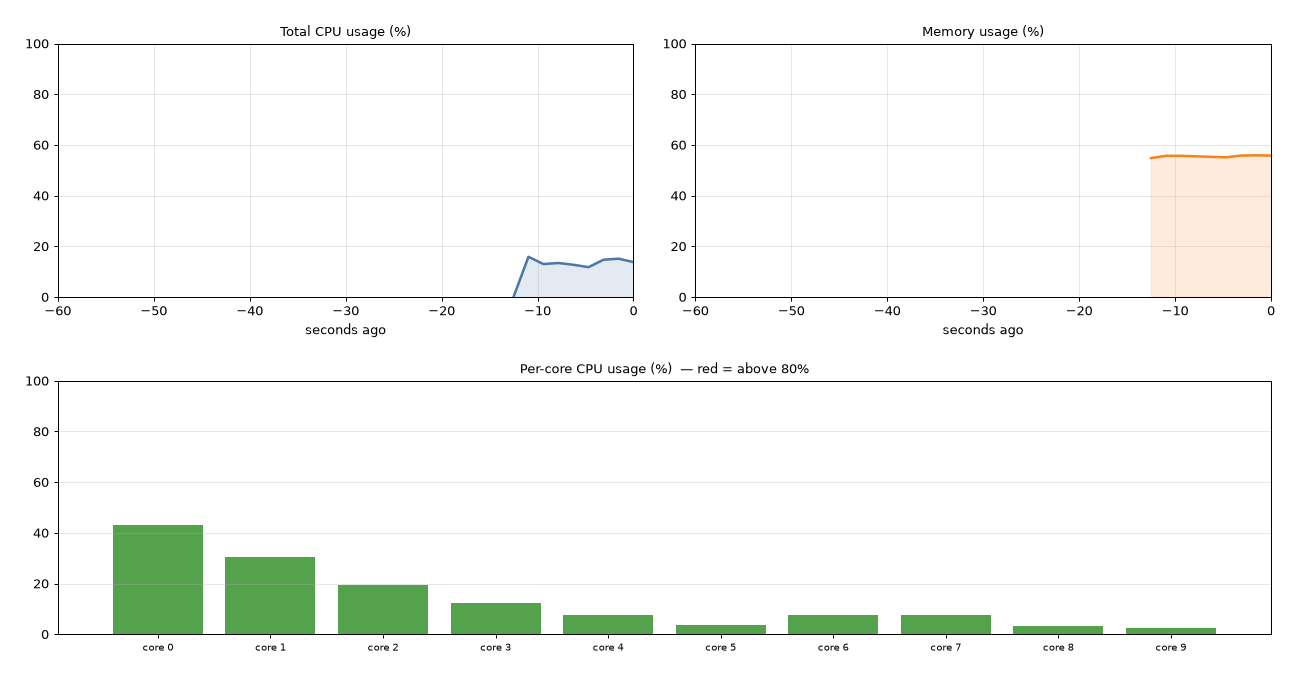
\includegraphics[width=0.95\textwidth]{system.png}
\caption{System Monitor tab: CPU and memory history and per-core usage.}
\end{figure}

%=======================================================================
\section{Results}

We used the following example, solved by hand first and then checked by our tests.
\begin{table}[H]
\centering
\begin{tabular}{cccc}
\toprule
Job & Arrival & Burst & Priority \\
\midrule
P1 & 0 & 5 & 3 \\ P2 & 1 & 3 & 2 \\ P3 & 2 & 1 & 1 \\
\bottomrule
\end{tabular}
\end{table}

\begin{table}[H]
\centering
\begin{tabular}{lcccc}
\toprule
Algorithm & Avg waiting & Avg turnaround & Avg response & Context switches \\
\midrule
FCFS & 3.33 & 6.33 & 3.33 & 2 \\
Priority (non-preemptive) & 2.67 & 5.67 & 2.67 & 2 \\
Priority (preemptive) & 1.67 & 4.67 & 0.00 & 4 \\
Round Robin ($q=2$) & 3.33 & 6.33 & 1.00 & 5 \\
\bottomrule
\end{tabular}
\caption{Results for the example.}
\end{table}

\begin{figure}[H]
\centering
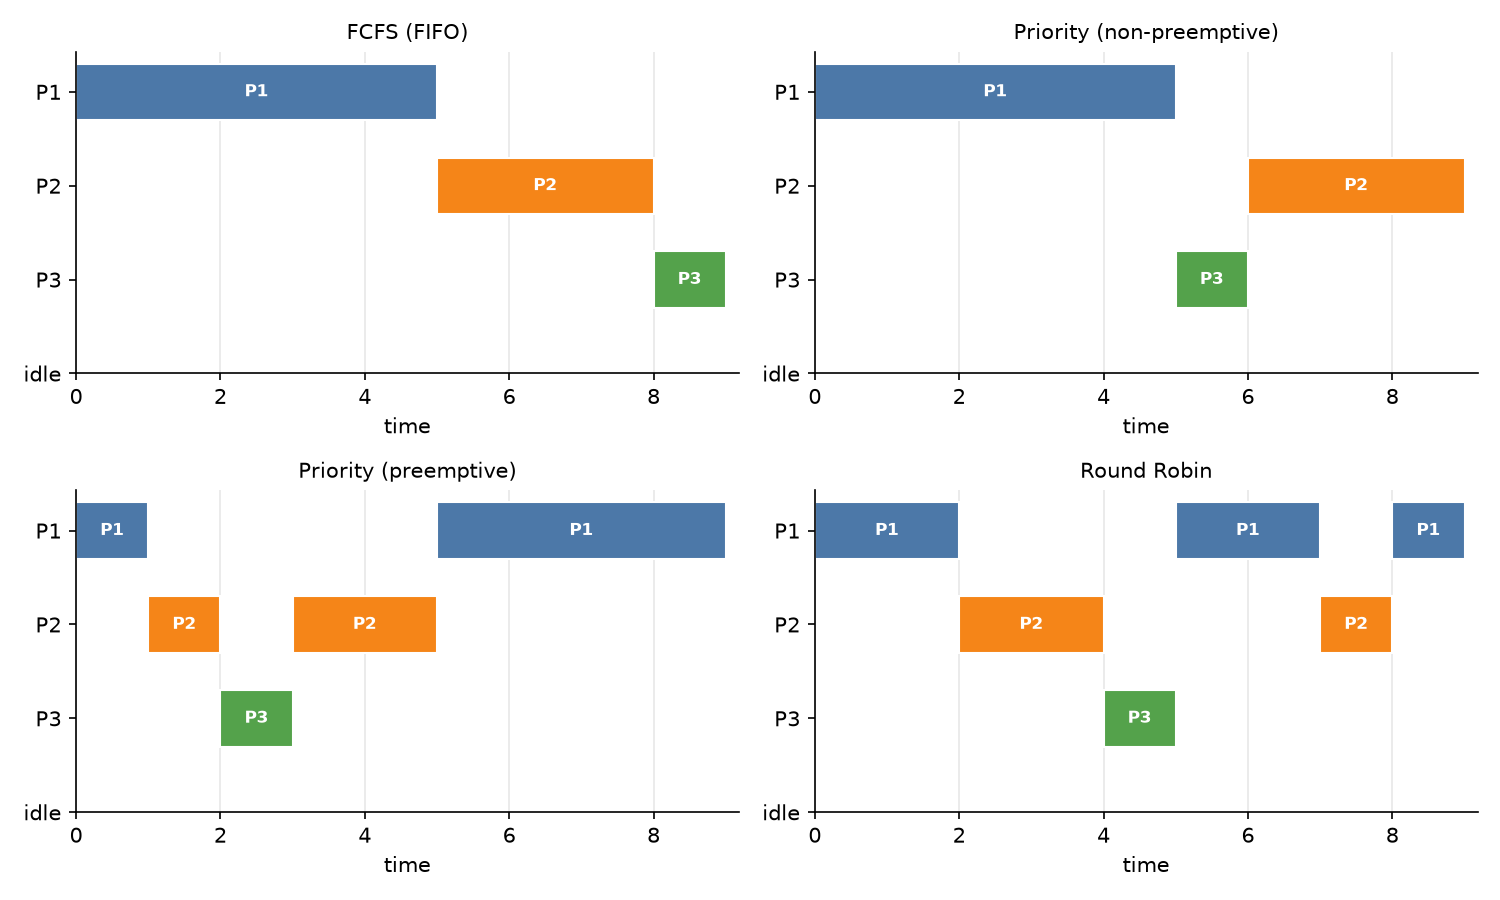
\includegraphics[width=\textwidth]{gantt_all.png}
\caption{Gantt charts of the four algorithms.}
\end{figure}

\begin{figure}[H]
\centering
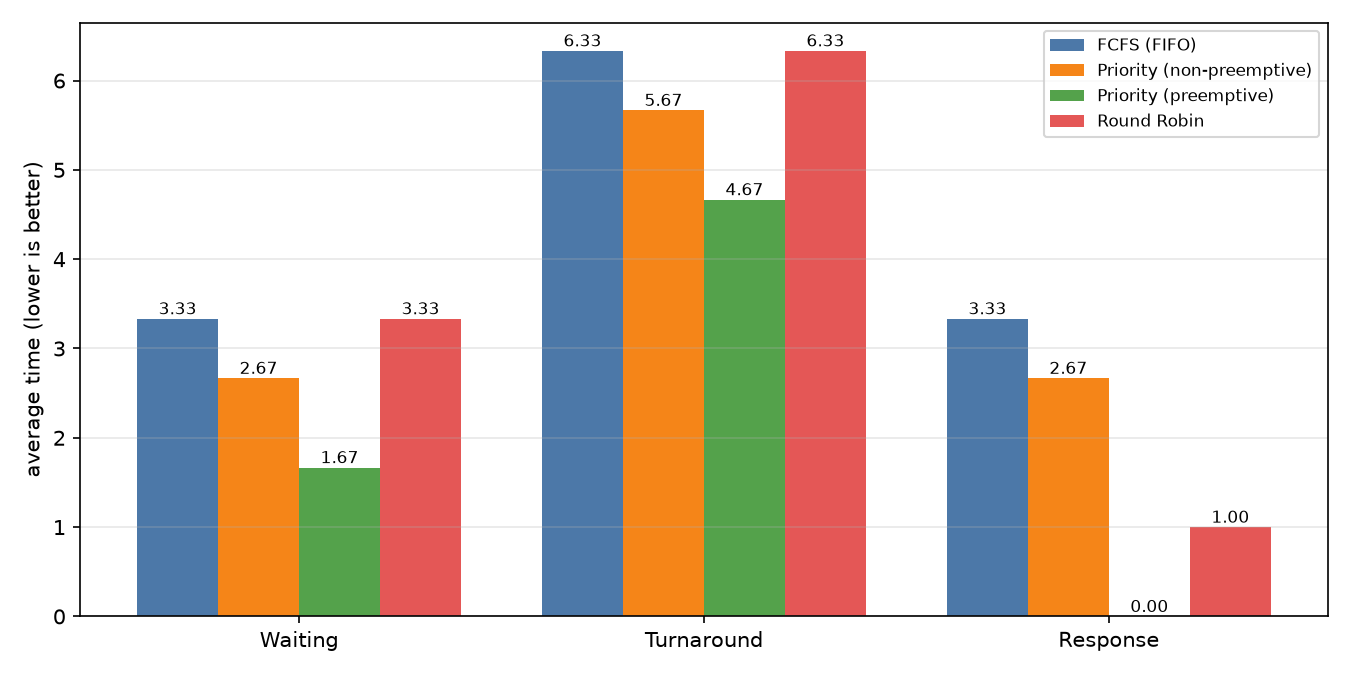
\includegraphics[width=0.85\textwidth]{compare.png}
\caption{Average waiting, turnaround and response time.}
\end{figure}

\textbf{Observations.} FCFS gives the worst response time because the short jobs wait
behind P1 (convoy effect). Round Robin has the same average waiting time as FCFS here but
gives every job its first turn much sooner (response 1.00 vs 3.33), at the cost of more
context switches. Preemptive priority is best for this input, but our test
\texttt{test\_starvation\_of\_low\_priority\_job} shows how it can make a low priority job wait
for a long time.

\begin{figure}[H]
\centering
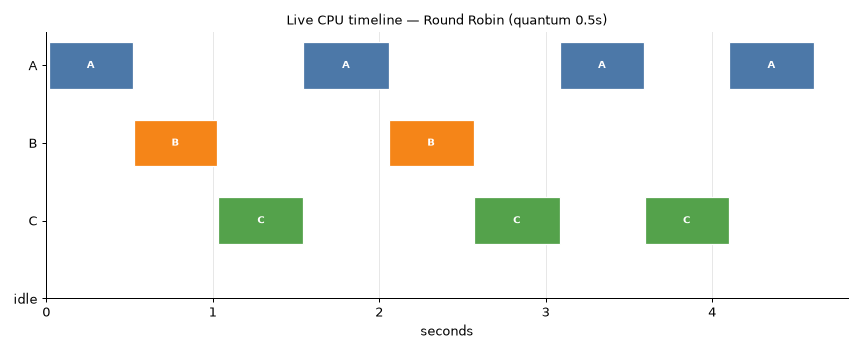
\includegraphics[width=0.95\textwidth]{real_rr.png}
\caption{Real child processes scheduled with Round Robin (quantum 0.5\,s).}
\end{figure}

%=======================================================================
\section{Testing}
We used Python's \texttt{unittest}. There are 26 tests:
\begin{itemize}
  \item every algorithm against hand-calculated results (order, finish times, averages);
  \item the fast heap-based priority code compared with a simple one-unit-at-a-time
        reference on 300 random job sets;
  \item edge cases: idle CPU gaps, a single job, equal priorities, quantum 1, convoy effect,
        starvation, invalid input;
  \item the monitor (our own PID appears in the tree with the correct parent);
  \item real processes scheduled with FCFS and Round Robin;
  \item the command line interface and its exit codes.
\end{itemize}
\texttt{scripts/run\_tests.sh} runs all unit tests plus six command-line checks and saves a log.

\begin{lstlisting}
$ ./scripts/run_tests.sh
Ran 26 tests in 1.6s
OK
PASS  compare all algorithms
PASS  round robin avg waiting
...
ALL TESTS PASSED
\end{lstlisting}

%=======================================================================
\section{Profiling}\label{sec:profiling}
We used \texttt{cProfile} and \texttt{pstats} (script \texttt{profiling/profile\_app.py},
run by \texttt{scripts/profile.sh}) on 3000 random jobs, and \texttt{/usr/bin/time -l} for
peak memory.

\subsection{Bottleneck 1: priority scheduling}
The first version was more than 100 times slower than FCFS and Round Robin. cProfile showed
6.2 million calls to the \texttt{min()} key function: at every step the code built a list
of ready jobs and searched all of it, which is $O(n^2)$.

\begin{lstlisting}[caption={cProfile output before the fix (shortened)}]
6241878 function calls in 0.823 seconds
 ncalls  tottime  cumtime  function
      1    0.277    0.824  scheduler.py(priority_preemptive)
  10485    0.304    0.533  {built-in method builtins.min}
6193222    0.229    0.229  scheduler.py(<lambda>)
\end{lstlisting}

\textbf{Fix:} sort the jobs by arrival once and keep the ready jobs in a heap
(\texttt{heapq}) ordered by (priority, arrival, input order). Taking the best job is now
$O(\log n)$.

\begin{figure}[H]
\centering
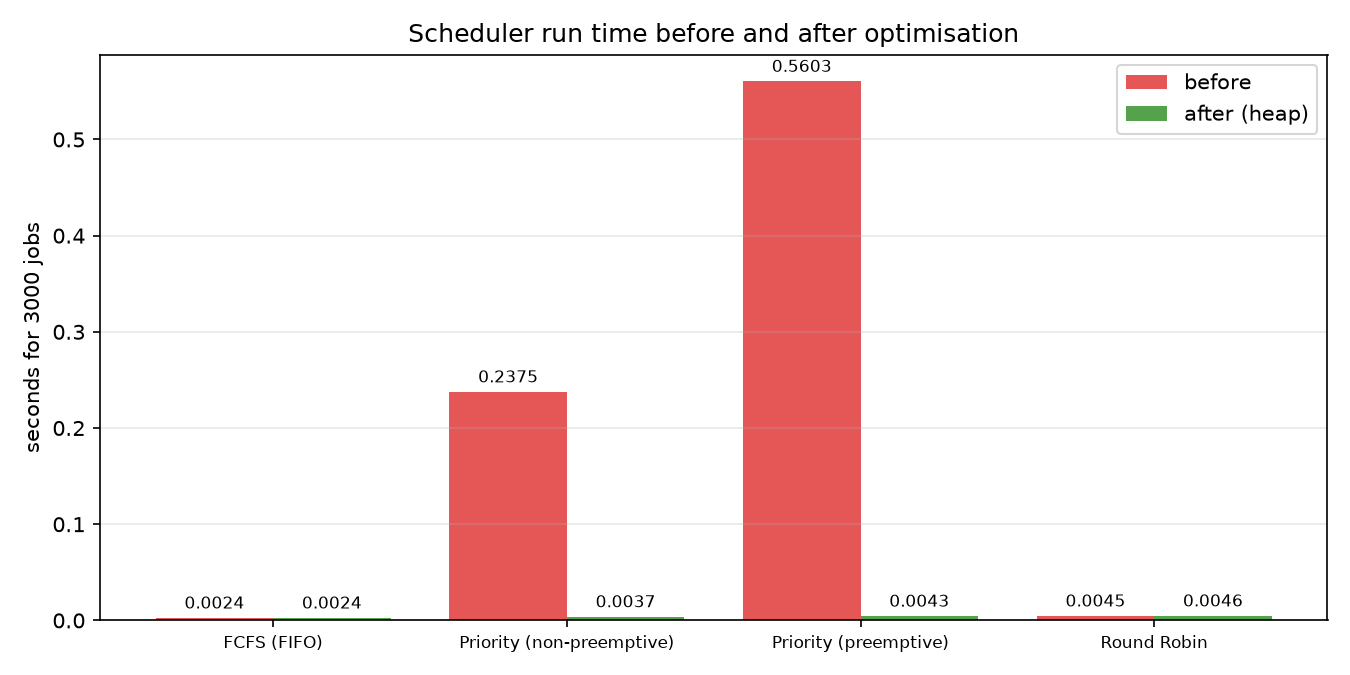
\includegraphics[width=0.85\textwidth]{profiling.png}
\caption{Run time before and after the optimisation (3000 jobs).}
\end{figure}

\begin{table}[H]
\centering
\begin{tabular}{lrrr}
\toprule
Algorithm & Before (s) & After (s) & Speed-up \\
\midrule
Priority (non-preemptive) & 0.2375 & 0.0036 & $\approx 66\times$ \\
Priority (preemptive) & 0.5603 & 0.0042 & $\approx 133\times$ \\
\bottomrule
\end{tabular}
\end{table}

\subsection{Bottleneck 2: user names in the monitor}
For one snapshot of about 670 processes, \texttt{pwd.getpwuid()} (turning a user id into a
name) took about a quarter of the time because psutil does it for every process. We read
the numeric uid instead and cache the names. Snapshot time went from 0.0244\,s to 0.0186\,s
(about 24\,\% faster).

%=======================================================================
\section{Automation with bash}
\begin{table}[H]
\centering
\begin{tabular}{lp{10.5cm}}
\toprule
Script & Purpose \\
\midrule
\texttt{setup.sh} & Finds a Python with Tk 8.6+, creates \texttt{.venv}, installs libraries \\
\texttt{run.sh} & Starts the GUI, or the CLI when arguments are given \\
\texttt{run\_tests.sh} & Unit tests + CLI checks, writes \texttt{tests/test\_log.txt}, exit code 0/1 \\
\texttt{profile.sh} & Runs cProfile, prints before/after timing and peak memory \\
\texttt{build\_docs.sh} & Compiles this report and the slides (latexmk, pdflatex or tectonic) \\
\texttt{stress.sh} & Starts CPU-heavy workers for the demo and kills them on exit (\texttt{trap}) \\
\texttt{demo.sh} & Step-by-step terminal demo for the presentation \\
\bottomrule
\end{tabular}
\end{table}

%=======================================================================
\section{Version control}
The project was developed with git; every feature, fix and document has its own commit.
The current history is:
\lstinputlisting{gitlog.txt}

%=======================================================================
\section{Problems we faced}
\begin{itemize}
  \item \textbf{GUI froze on macOS.} Apple's built-in Python ships Tk 8.5, which hangs on
        recent macOS. We switched to Homebrew's Python with Tk 9, and \texttt{setup.sh} now
        checks the Tk version.
  \item \textbf{Permission errors.} Some system processes hide fields; psutil returns
        \texttt{None} for them instead of crashing.
  \item \textbf{Thread safety.} Updating Tk widgets from a background thread is unsafe, so
        threads only share data through a lock and a queue.
  \item \textbf{First CPU reading is 0.} psutil needs two readings to compute CPU\%, so we
        skip the first sample.
\end{itemize}

%=======================================================================
\section{Conclusion and future work}
The application monitors processes, shows the process hierarchy, plots system usage and
compares scheduling algorithms on both simulated and real processes. Profiling helped
us find and remove a real $O(n^2)$ bottleneck. Possible extensions: Shortest Job First
and multilevel feedback queues, aging for priority scheduling, and saving monitoring
history to a file.

%=======================================================================
\section{Team contribution}
\begin{table}[H]
\centering
\begin{tabular}{lp{10cm}}
\toprule
Member & Work \\
\midrule
Rahul Ahirwar
\bottomrule
\end{tabular}
\end{table}

%=======================================================================
\section{Declaration of AI use}
As allowed by the course AI policy, we used an AI assistant (Claude, by Anthropic) while
building this project. It helped us plan the project, explain the concepts, write first
versions of the code, the scripts and this report, and set up profiling. We reviewed and
ran all of the code and checked the scheduling results by hand. Every team member
can explain the parts listed under their name. All profiling numbers and test results in
this report come from running the project on our own machine.

%=======================================================================
\begin{thebibliography}{9}
\bibitem{ostep} R. Arpaci-Dusseau and A. Arpaci-Dusseau, \emph{Operating Systems: Three Easy Pieces}, chapters on scheduling.
\bibitem{galvin} A. Silberschatz, P. Galvin, G. Gagne, \emph{Operating System Concepts}, Wiley.
\bibitem{psutil} psutil documentation, \url{https://psutil.readthedocs.io}
\bibitem{pyprof} Python documentation, \emph{The Python Profilers}, \url{https://docs.python.org/3/library/profile.html}
\bibitem{mpl} matplotlib documentation, \url{https://matplotlib.org}
\end{thebibliography}

\end{document}

